%% smpost/thumbnail/chapter_09_crossing_the_border.tex : thumbnail of video 9/30,
%% "Chapter-9 | The Hand-over Drop at the Border: Geant4 Primaries". Motif: the
%% gate of the film's first scene. Three streams walk in from the left, the
%% family (red), the in-time crowd (grey) and the out-of-time crowd (gold);
%% at the gate the members that are not handed over fall out of the stream,
%% and the rest gather at the centre of the detector, drawn as the barrel of
%% CMS seen along the beam: tracker, ECAL, HCAL, solenoid, iron.
%% Compile: make thumbnails-youtube   (or: pdflatex chapter_09_crossing_the_border)
\documentclass[tikz,border=0pt]{standalone}
%% ==========================================================================
%% smpost/thumbnail/thumbnail_common.tex : what every JitJet video thumbnail
%% shares. Each chapter_XX_*.tex in this directory is a standalone TikZ
%% document that \input{}s this file after \documentclass and then draws its
%% own motif on the right of the page.
%%
%% The page is 19.2 cm x 10.8 cm, i.e. 1280 x 720 px at 1 px = 0.015 cm, the
%% YouTube thumbnail size (16:9). `make thumbnails-youtube` compiles every
%% chapter_*.tex here and rasterises it with gs to a 1280 x 720 PNG.
%%
%% Layout: the wordmark top left, the "n / 30" pill top right, the stop number
%% in a milestone ring with the chapter label, the title in two big lines and
%% the subtitle under it, all in the left 10 cm; the motif of the chapter sits
%% in the right part, centred on (\mx, \my), inside about 8 cm x 8 cm, over a
%% soft gold glow.
%%   \thumbbackground
%%   \thumbtext{<stop number>}{<chapter label>}{<n / 30>}{<title, with \\>}{<subtitle>}
%% ==========================================================================
\usepackage[T1]{fontenc}
\usepackage{lmodern}
\usepackage{tgheros}          % TeX Gyre Heros, as on the cover
\usepackage{amssymb}
\usetikzlibrary{calc,arrows.meta,decorations.pathmorphing,decorations.markings,shapes.geometric}
\hyphenpenalty=10000 \exhyphenpenalty=10000   % no hyphens in titles and subtitles

%% -------- palette (identical to cover.tex) ----------------------------------
\definecolor{navy}{HTML}{0B1D3A}
\definecolor{navytop}{HTML}{17365F}
\definecolor{gold}{HTML}{F4B942}
\definecolor{bred}{HTML}{FF5A5A}     % b quark
\definecolor{bblue}{HTML}{6E8EFF}    % bbar
\definecolor{fsr}{HTML}{3DD16E}      % FSR gluons
\definecolor{isr}{HTML}{FF9A3C}      % ISR gluon
\definecolor{hadroncol}{HTML}{FFC24D}
\definecolor{ecalcol}{HTML}{3FBF77}
\definecolor{hcalcol}{HTML}{E58F2A}
\definecolor{steel}{HTML}{9AA7B8}
\definecolor{trackcol}{HTML}{E4ECF7}
\definecolor{pu}{HTML}{8D9AAB}
\definecolor{nucol}{HTML}{5EE7EA}
\definecolor{muoncol}{HTML}{8FB8FF}

%% -------- the cone of the cover, for thumbnails that show it ----------------
\def\kk{0.30}
\pgfmathdeclarefunction{rf}{1}{\pgfmathparse{0.18*#1+0.6*(1+((#1-16.8)/1.2)/sqrt(1+((#1-16.8)/1.2)^2))}}
\pgfmathdeclarefunction{sc}{1}{\pgfmathparse{min(rf(#1)/2.2,1)}}
\newcommand{\xy}[3]{({#1+\kk*#2*sc(#1)*cos(#3)},{#2*sc(#1)*sin(#3)})}
\newcommand{\xring}[2]{%
  \draw[ringback] ({#1},{#2}) arc[start angle=90, end angle=-90, x radius={\kk*#2}, y radius={#2}];
  \draw[ring]     ({#1},{#2}) arc[start angle=90, end angle=270, x radius={\kk*#2}, y radius={#2}];}
\newcommand{\xellipse}[3][]{\path[#1] ({#2},0) ellipse [x radius={\kk*#3}, y radius={#3}];}

%% -------- where the motif goes ----------------------------------------------
\def\mx{14.6}
\def\my{5.3}

%% -------- styles ------------------------------------------------------------
\tikzset{
  ring/.style={draw=gold!75!white, line width=0.6pt, opacity=0.9},
  ringback/.style={draw=white, line width=0.4pt, opacity=0.3, dash pattern=on 1pt off 1pt},
  meridian/.style={draw=white, line width=0.3pt, opacity=0.15},
  edge/.style={draw=gold!80!white, line width=1.1pt},
  bline/.style={draw=bred, line width=3pt, line cap=round},
  bbarline/.style={draw=bblue, line width=3pt, line cap=round},
  qline/.style={draw=trackcol, line width=2pt, line cap=round},
  gluon/.style={draw=fsr, line width=1.6pt, decorate,
    decoration={coil, aspect=0.6, segment length=4pt, amplitude=2.6pt}},
  isrgluon/.style={gluon, draw=isr},
  quark/.style={draw=hadroncol, line width=1.6pt, line cap=round},
  string/.style={draw=hadroncol, line width=2.4pt, line cap=round},
  hadron/.style={circle, fill=hadroncol, draw=navy, line width=0.6pt, inner sep=0pt, minimum size=9pt},
  track/.style={draw=trackcol, line width=1.3pt, line cap=round},
  pudot/.style={circle, fill=pu, inner sep=0pt, minimum size=4pt, opacity=0.8},
  pf/.style={circle, inner sep=0pt, minimum size=5pt, draw=navy, line width=0.3pt},
  roadline/.style={draw=gold, line width=1.4pt, dash pattern=on 7pt off 5pt},
  milestone/.style={circle, draw=gold, fill=navy, line width=1.6pt, minimum size=26pt,
    inner sep=0pt, font=\sffamily\bfseries\large, text=gold},
  mlabel/.style={font=\sffamily\bfseries, text=white, align=center, inner sep=4pt,
    fill=navy, rounded corners=2pt, draw=gold, line width=0.8pt},
  flight/.style={draw=bred, line width=1.4pt, dash pattern=on 4pt off 3pt},
  vertex/.style={circle, draw=bred, fill=navy, line width=1.6pt, inner sep=0pt, minimum size=9pt},
  arrowg/.style={-{Stealth[length=7pt]}, draw=gold, line width=1.2pt},
  motiflabel/.style={font=\sffamily\bfseries\small, inner sep=1.5pt},
}

%% -------- the page ----------------------------------------------------------
\newcommand{\thumbbackground}{%
  \useasboundingbox (0,0) rectangle (19.2,10.8);
  \clip (0,0) rectangle (19.2,10.8);
  \shade[top color=navytop, bottom color=navy!80!black] (0,0) rectangle (19.2,10.8);
  \draw[white, opacity=0.045, line width=0.3pt, step=1cm] (0,0) grid (19.2,10.8);
  \shade[inner color=gold, outer color=navy, opacity=0.16] (\mx,\my) circle[radius=4.6];
  \draw[gold, line width=0.6pt, opacity=0.8] (0.9,0.85) -- (18.3,0.85);
  \node[anchor=south west, gold!80!white, font=\sffamily\scriptsize] at (0.9,0.95) {Journey Is The Jet \,$\cdot$\, bottom to top};
  \node[anchor=south east, white!70!navy, font=\sffamily\scriptsize] at (18.3,0.95) {github.com/ravindkv/JitJet};
}

%% \thumbtext{stop}{chapter label}{n / 30}{title}{subtitle}
\newcommand{\thumbtext}[5]{%
  \node[anchor=west] at (0.9,9.65)
    {\fontsize{26}{28}\selectfont\sffamily\bfseries{\color{white}Jit}{\color{gold}Jet}};
  \node[anchor=east, gold, font=\sffamily\bfseries\small, draw=gold, line width=0.8pt,
        rounded corners=6pt, inner xsep=7pt, inner ysep=3.5pt] at (18.3,9.65) {#3};
  \node[milestone] (stop) at (1.45,7.85) {#1};
  \node[anchor=west, gold, font=\fontsize{15}{17}\selectfont\sffamily\scshape] at (2.1,7.85) {#2};
  \node[anchor=north west, white, align=left, inner sep=0pt,
        font=\fontsize{34}{39}\selectfont\sffamily\bfseries] (ttl) at (0.9,7.05) {#4};
  \node[anchor=north west, gold!90!white, align=left, inner sep=0pt, text width=9.6cm,
        font=\fontsize{14}{17}\selectfont\sffamily\itshape] at ($(ttl.south west)+(0,-0.4)$) {#5};
}

\begin{document}
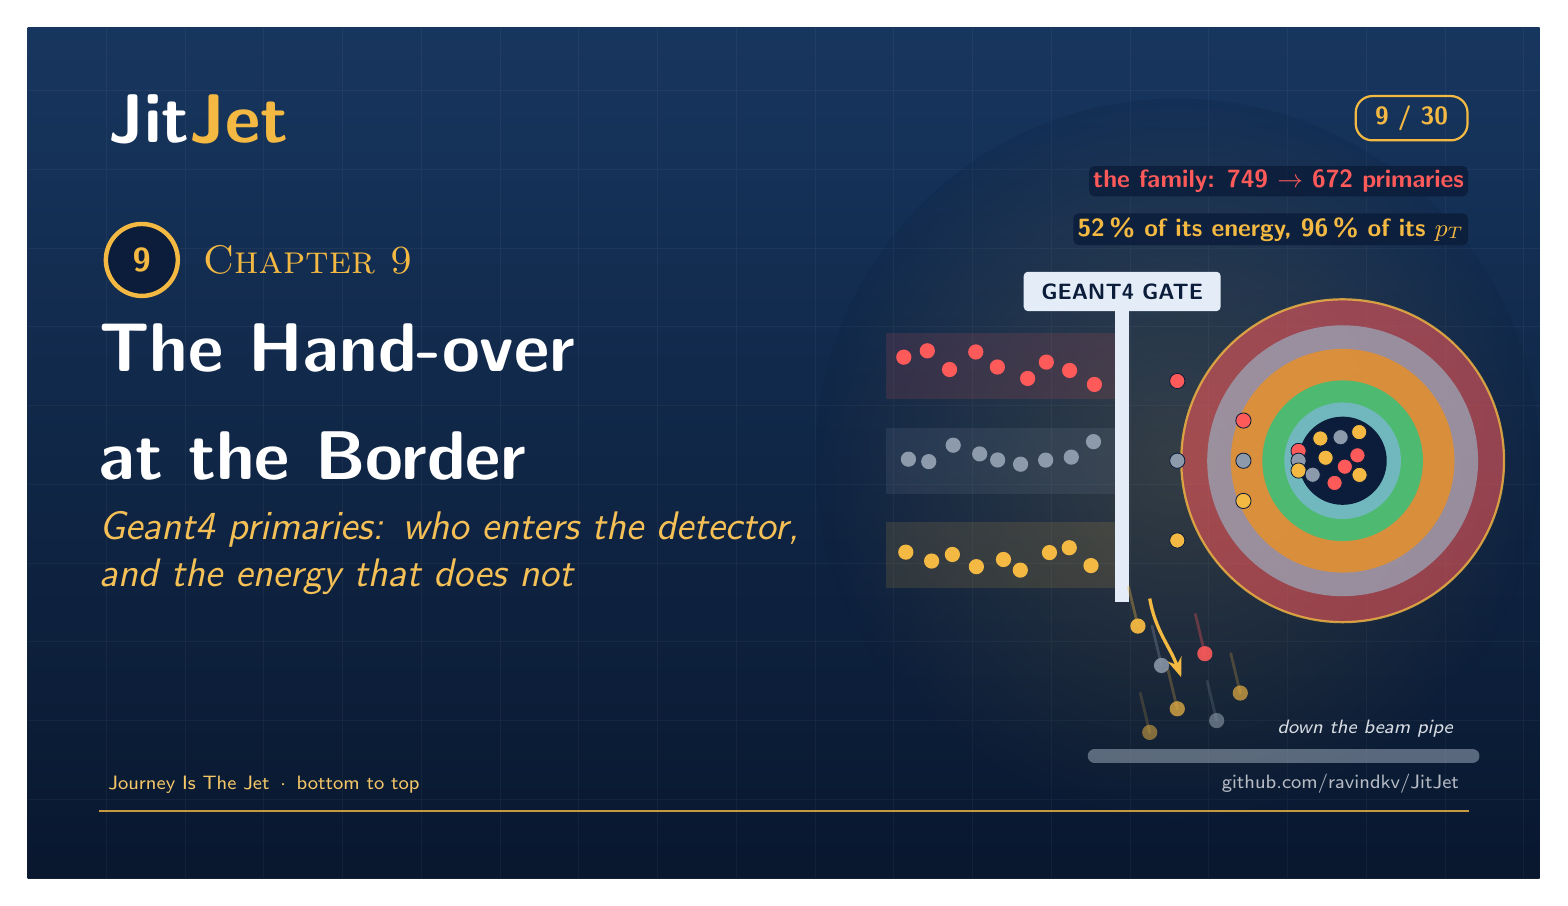
\begin{tikzpicture}[x=1cm,y=1cm]
\thumbbackground
\thumbtext{9}{Chapter 9}{9 / 30}{The Hand-over\\at the Border}{Geant4 primaries: who enters the detector, and the energy that does not}

\begin{scope}[shift={(\mx+0.15,\my-0.55)}]
\def\gx{-0.85}    % the gate
\def\cx{1.95}     % the centre of the detector
\def\cy{0.55}
%% the detector behind the gate: the barrel seen along the beam
\foreach \r/\c/\o in {2.05/bred/0.55, 1.72/steel/0.75, 1.42/hcalcol/0.85, 1.02/ecalcol/0.9, 0.74/muoncol/0.55}
  \fill[\c, opacity=\o] (\cx,\cy) circle[radius=\r];
\fill[navy] (\cx,\cy) circle[radius=0.56];
\draw[gold, line width=0.8pt, opacity=0.8] (\cx,\cy) circle[radius=2.05];
%% the three lanes
\foreach \y/\c in {1.75/bred, 0.55/pu, -0.65/gold}
  \fill[\c, opacity=0.13] (-3.85,\y-0.42) rectangle (\gx,\y+0.42);
%% the streams: dots walking towards the gate
\pgfmathsetseed{9}
\foreach \y/\c in {1.75/bred, 0.55/pu, -0.65/gold}{
  \foreach \i in {1,...,9}{
    \pgfmathsetmacro{\xx}{-3.95+0.3*\i+0.1*rnd}
    \pgfmathsetmacro{\yy}{\y+0.5*(rnd-0.5)}
    \node[circle, fill=\c, inner sep=0pt, minimum size=5.5pt] at (\xx,\yy) {};}}
%% the gate
\fill[trackcol] (\gx-0.09,-1.25) rectangle (\gx+0.09,2.45);
\fill[trackcol, rounded corners=1.5pt] (\gx-1.25,2.45) rectangle (\gx+1.25,2.95);
\node[navy, font=\sffamily\bfseries\footnotesize] at (\gx,2.7) {GEANT4 GATE};
%% the handed over: from the gate to the centre of the detector
\foreach \y/\c in {1.75/bred, 0.55/pu, -0.65/gold}{
  \foreach \u in {0.25,0.55,0.8}{
    \pgfmathsetmacro{\xx}{\gx+(\cx-\gx)*\u}
    \pgfmathsetmacro{\yy}{\y+(\cy-\y)*\u*\u*(3-2*\u)}
    \node[circle, fill=\c, draw=navy, line width=0.3pt, inner sep=0pt, minimum size=5.5pt] at (\xx,\yy) {};}}
\foreach \a/\r/\c in {20/0.2/bred, 95/0.3/pu, 170/0.22/gold, 250/0.3/bred, 320/0.28/gold, 60/0.42/gold, 205/0.42/pu, 290/0.08/bred, 135/0.4/gold}
  \node[circle, fill=\c, draw=navy, line width=0.3pt, inner sep=0pt, minimum size=5.5pt] at ($(\cx,\cy)+(\a:\r)$) {};
%% the dropped: falling out of the stream at the gate
\foreach \x/\y/\c/\o in {-0.65/-1.55/gold/0.95, -0.35/-2.05/pu/0.85, -0.15/-2.6/gold/0.7, 0.2/-1.9/bred/0.9, 0.35/-2.75/pu/0.6, -0.5/-2.9/gold/0.5, 0.65/-2.4/gold/0.65}{
  \draw[\c, opacity=0.35*\o, line width=1pt, line cap=round] (\x-0.12,\y+0.5) -- (\x,\y);
  \node[circle, fill=\c, opacity=\o, inner sep=0pt, minimum size=5.5pt] at (\x,\y) {};}
\draw[arrowg] (\gx+0.35,-1.2) to[out=-80,in=110] (\gx+0.75,-2.2);
%% the beam pipe the dropped go down
\draw[steel, line width=5pt, line cap=round, opacity=0.55] (-1.2,-3.2) -- (3.6,-3.2);
\node[steel!40!white, font=\sffamily\scriptsize\itshape, anchor=west] at (1.0,-2.85) {down the beam pipe};
\end{scope}
%% the numbers to take away
\node[bred, motiflabel, anchor=north east, fill=navy, fill opacity=0.85, text opacity=1, rounded corners=2pt, align=right] at (18.3,9.05)
  {the family: 749 $\to$ 672 primaries};
\node[gold, motiflabel, anchor=north east, fill=navy, fill opacity=0.85, text opacity=1, rounded corners=2pt, align=right] at (18.3,8.45)
  {52\,\% of its energy, 96\,\% of its $p_T$};
\end{tikzpicture}
\end{document}
